\documentclass[a4paper,14pt,oneside,final]{extarticle}
\usepackage[top=2cm, bottom=2cm, left=3cm, right=1cm]{geometry}
\usepackage{scrextend}

\usepackage[T2A,T1]{fontenc}
\usepackage[ukrainian,russian,english]{babel}
\usepackage{tempora}
\usepackage{fontspec}
\setmainfont{tempora}

% Зачем: Отключает использование изменяемых межсловных пробелов.
% Почему: Так не принято делать в текстах на русском языке.
\frenchspacing

\usepackage{indentfirst}
\setlength{\parindent}{1.25cm}
\renewcommand{\baselinestretch}{1.5}

% Header
\usepackage{fancyhdr}
\pagestyle{fancy}
\fancyhead{}
\fancyfoot{}
\fancyhead[R]{\small \selectfont \thepage}
\renewcommand{\headrulewidth}{0pt}

% Captions
\usepackage{chngcntr}
\counterwithin{figure}{section}
\counterwithin{table}{section}
\usepackage[tableposition=top]{caption}
\usepackage{subcaption}
\DeclareCaptionLabelFormat{gostfigure}{Рисунок #2}
\DeclareCaptionLabelFormat{gosttable}{Таблиця #2}
\DeclareCaptionLabelSeparator{gost}{~---~}
\captionsetup{labelsep=gost}
\captionsetup[figure]{labelformat=gostfigure}
\captionsetup[table]{labelformat=gosttable}
\renewcommand{\thesubfigure}{\asbuk{subfigure}}

% Sections
\usepackage[explicit]{titlesec}
\newcommand{\sectionbreak}{\clearpage}

\titleformat{\section}
  {\centering}{\thesection \quad}{0pt}{\MakeUppercase{#1}}
\titleformat{\subsection}[block]
  {\bfseries}{\thesubsection \quad #1}{0cm}{}

\titlespacing{\section} {0cm}{0cm}{21pt}
\titlespacing{\subsection} {\parindent}{21pt}{0cm}
\titlespacing{\subsubsection} {\parindent}{0cm}{0cm}

% Lists
\usepackage{enumitem}
\renewcommand\labelitemi{--}
\setlist[itemize]{noitemsep, topsep=0pt, wide}
\setlist[enumerate]{noitemsep, topsep=0pt, wide, label=\arabic*}
\setlist[description]{labelsep=0pt, noitemsep, topsep=0pt, leftmargin=2\parindent, labelindent=\parindent, labelwidth=\parindent, font=\normalfont}

% Toc
\usepackage{tocloft}
\tocloftpagestyle{fancy}
\renewcommand{\cfttoctitlefont}{}
\setlength{\cftbeforesecskip}{0pt}
\renewcommand{\cftsecfont}{}
\renewcommand{\cftsecpagefont}{}
\renewcommand{\cftsecleader}{\cftdotfill{\cftdotsep}}

\usepackage{float}
\usepackage{pgfplots}
\usepackage{graphicx}
\usepackage{multirow}
\usepackage{amssymb,amsfonts,amsmath,amsthm}
\usepackage{csquotes}

\usepackage{listings}
\lstset{basicstyle=\footnotesize\ttfamily,breaklines=true}
\lstset{language=Matlab}

\usepackage[
	backend=biber,
	sorting=none,
	language=auto,
	autolang=other
]{biblatex}
\DeclareFieldFormat{labelnumberwidth}{#1}


\newcommand{\labnumber}{1} % first lab
\documentclass[a4paper,14pt,oneside,final]{extarticle}
\usepackage[top=2cm, bottom=2cm, left=3cm, right=1cm]{geometry}
\usepackage{scrextend}

\usepackage[T2A,T1]{fontenc}
\usepackage[ukrainian,russian,english]{babel}
\usepackage{tempora}
\usepackage{fontspec}
\setmainfont{tempora}

% Зачем: Отключает использование изменяемых межсловных пробелов.
% Почему: Так не принято делать в текстах на русском языке.
\frenchspacing

\usepackage{indentfirst}
\setlength{\parindent}{1.25cm}
\renewcommand{\baselinestretch}{1.5}

% Header
\usepackage{fancyhdr}
\pagestyle{fancy}
\fancyhead{}
\fancyfoot{}
\fancyhead[R]{\small \selectfont \thepage}
\renewcommand{\headrulewidth}{0pt}

% Captions
\usepackage{chngcntr}
\counterwithin{figure}{section}
\counterwithin{table}{section}
\usepackage[tableposition=top]{caption}
\usepackage{subcaption}
\DeclareCaptionLabelFormat{gostfigure}{Рисунок #2}
\DeclareCaptionLabelFormat{gosttable}{Таблиця #2}
\DeclareCaptionLabelSeparator{gost}{~---~}
\captionsetup{labelsep=gost}
\captionsetup[figure]{labelformat=gostfigure}
\captionsetup[table]{labelformat=gosttable}
\renewcommand{\thesubfigure}{\asbuk{subfigure}}

% Sections
\usepackage[explicit]{titlesec}
\newcommand{\sectionbreak}{\clearpage}

\titleformat{\section}
  {\centering}{\thesection \quad}{0pt}{\MakeUppercase{#1}}
\titleformat{\subsection}[block]
  {\bfseries}{\thesubsection \quad #1}{0cm}{}

\titlespacing{\section} {0cm}{0cm}{21pt}
\titlespacing{\subsection} {\parindent}{21pt}{0cm}
\titlespacing{\subsubsection} {\parindent}{0cm}{0cm}

% Lists
\usepackage{enumitem}
\renewcommand\labelitemi{--}
\setlist[itemize]{noitemsep, topsep=0pt, wide}
\setlist[enumerate]{noitemsep, topsep=0pt, wide, label=\arabic*}
\setlist[description]{labelsep=0pt, noitemsep, topsep=0pt, leftmargin=2\parindent, labelindent=\parindent, labelwidth=\parindent, font=\normalfont}

% Toc
\usepackage{tocloft}
\tocloftpagestyle{fancy}
\renewcommand{\cfttoctitlefont}{}
\setlength{\cftbeforesecskip}{0pt}
\renewcommand{\cftsecfont}{}
\renewcommand{\cftsecpagefont}{}
\renewcommand{\cftsecleader}{\cftdotfill{\cftdotsep}}

\newcommand{\khpistudentgroup}{КН-34г}
\newcommand{\khpistudentname}{Чепурний~А.~С.}

\newcommand{\khpidepartment}{Програмна інженерія та інформаційні технології управління}
\newcommand{\khpititlewhat}{
	Лабораторна робота №\labnumber \\
	з предмету <<Моделювання систем>>
}
\newcommand{\khpititlewho}{
	Виконав: \\
	\hspace*{\parindent} ст. групи \khpistudentgroup \\
	\hspace*{\parindent} \khpistudentname \\
	Перевірила: \\
	\hspace*{\parindent} ст. в. каф. ПІІТУ \\
	\hspace*{\parindent} Єршова~С.~І. \\
	\hspace*{\parindent} ас. каф. ПІІТУ \\
	\hspace*{\parindent} Литвинова~Ю.~С. \\
}



\usepackage{systeme}
\usepackage{longtable,tabu}
\usepackage{multirow}
\usepackage{array,multirow}
\usepackage{pdflscape}
\usepackage{afterpage}
\usepackage{bm}

\graphicspath{{../figures/}}

\begin{document}
\Ukrainian

\begin{titlepage}

\begin{center}
	МІНІСТЕРСТВО ОСВІТИ І НАУКИ УКРАЇНИ \\
	НАЦІОНАЛЬНИЙ ТЕХНІЧНИЙ УНІВЕРСИТЕТ \\
	«ХАРКІВСЬКИЙ ПОЛІТЕХНІЧНИЙ ІНСТИТУТ» \\[0.5cm]
	Кафедра <<\khpidepartment>> \\
\end{center}

\vspace{6cm}

\begin{center}
	\khpititlewhat
\end{center}

\vspace{3cm}

\begin{addmargin}[10cm]{0cm}
	\khpititlewho
\end{addmargin}

\vspace{\fill}

\begin{center}
	Харків \the\year
\end{center}

\end{titlepage}

\addtocounter{page}{1}

\textbf{Тема роботи}: розв'язання багатокритеріальної задачі щодо знаходження ефективних альтернатив за допомогою теореми Карліна.

\textbf{Завдання для виконання}: вирішити наступну задачу багатокритеріальної оптимізації:
Вариант №1

\begin{align*}
k_{u_1}=0.68, k_{u_2}=0.83.
\end{align*}

{
	\small
	\tabulinesep=1.2mm
	\begin{longtabu} to \textwidth {|X[12,l]|X[1,c]X[1,c]X[1,c]|X[1,c]X[1,c]X[1,c]|X[1,c]X[1,c]X[1,c]|X[1,c]X[1,c]X[1,c]|X[1,c]X[1,c]X[1,c]|}  
		\caption{Самооценка экспертов}
		\label{tab:selfscore} \\
		\hline
		\multirow{3}{*}{Источник аргументации} & \multicolumn{15}{c|}{Уровень влияния источника на мнение эксперта} \\ \cline{2-16}
		& \multicolumn{3}{c|}{Эксперт 1} & \multicolumn{3}{c|}{Эксперт 2} & \multicolumn{3}{c|}{Эксперт 3} & \multicolumn{3}{c|}{Эксперт 4} & \multicolumn{3}{c|}{Эксперт 5} \\ \cline{2-16}
		& A & B & C & A & B & C & A & B & C & A & B & C & A & B & C \\ \hline
		\endfirsthead

		\caption*{Окончание таблицы \thetable{}}\\
	    \hline
		\multirow{3}{*}{Источник аргументации} & \multicolumn{15}{c|}{Уровень влияния источника на мнение эксперта} \\ \cline{2-16}
		& \multicolumn{3}{c|}{Эксперт 1} & \multicolumn{3}{c|}{Эксперт 2} & \multicolumn{3}{c|}{Эксперт 3} & \multicolumn{3}{c|}{Эксперт 4} & \multicolumn{3}{c|}{Эксперт 5} \\ \cline{2-16}
		& A & B & C & A & B & C & A & B & C & A & B & C & A & B & C \\ \hline
		\endhead

	 	Проведенный экспертом теоретический анализ данной проблемы 
		& & \checkmark & & & \checkmark & & & \checkmark & & \checkmark & & & & & \checkmark \\ \hline
		Производственный опыт эксперта, связанный с решаемой проблемой & \checkmark & & & & \checkmark & & & \checkmark & & & \checkmark & & & & \checkmark \\ \hline
		Участие в семинарах, совещаниях в своей стране по исследуемой проблеме & & & \checkmark & & & \checkmark & \checkmark & & & & \checkmark & & & \checkmark & \\ \hline
		Знакомство с работами зарубежных авторов по рассматриваемой проблеме & & & \checkmark & & & \checkmark & \checkmark & & & & & \checkmark & & \checkmark & \\ \hline
		Количество проектов, в подготовке, реализации и экспертизе которых эксперт принимал участие & & \checkmark & & & \checkmark & & & \checkmark & & \checkmark & & & & & \checkmark \\ \hline
		Влияние интуиции эксперта на принимаемые решения & & \checkmark & & \checkmark & & & & \checkmark & & & \checkmark & & \checkmark & & \\ \hline
	\end{longtabu}
}

{
	\small
	\tabulinesep=1.2mm
	\begin{longtabu} to \textwidth {|X[1,c]|X[1,c]|X[1,c]|X[1,c]|X[1,c]|X[1,c]|X[1,c]|}  
		\caption{Параметры экспертов}
		\label{tab:score} \\
		\hline
		$k_i$  & $u$ & Эксперт 1 & Эксперт 2 & Эксперт 3 & Эксперт 4 & Эксперт 5 \\ \hline
		\endfirsthead

		\caption*{Окончание таблицы \thetable{}}\\
	    \hline
		$k_i$  & $u$ & Эксперт 1 & Эксперт 2 & Эксперт 3 & Эксперт 4 & Эксперт 5 \\ \hline
		\endhead

	 	$0.0003$ & $u_{lt} $ & $34$ & $26$ & $52$ & $41$ & $60$ \\ \hline
	 	$0.0008$ & $u_{sm} $ & $2$ & $14$ & $15$ & $3$ & $16$ \\ \hline
	 	$0.0015$ & $u_{sd} $ & $16$ & $3$ & $20$ & $21$ & $12$ \\ \hline
	 	$0.0020$ & $u_{z3} $ & $12$ & $14$ & $2$ & $2$ & $32$ \\ \hline
	 	$0.0010$ & $u_{z5} $ & $16$ & $23$ & $24$ & $10$ & $39$ \\ \hline
	 	$0.0009$ & $u_{zsp} $ & $5$ & $2$ & $14$ & $8$ & $9$ \\ \hline
	 	$0.0010$ & $u_{zv} $ & $26$ & $7$ & $2$ & $20$ & $32$ \\ \hline
	 	$0.0015$ & $u_{vs} $ & $5$ & $12$ & $5$ & $2$ & $3$ \\ \hline
	 	$0.0020$ & $u_{vz} $ & $1$ & $2$ & $4$ & $7$ & $0$ \\ \hline
	 	$0.0033$ & $u_{vsp} $ & $18$ & $23$ & $7$ & $21$ & $5$ \\ \hline
	 	$0.0080$ & $u_{zdl} $ & $4$ & $3$ & $5$ & $5$ & $4$ \\ \hline
	 	$0.0070$ & $u_{dlz} $ & $4$ & $3$ & $4$ & $4$ & $4$ \\ \hline
	 	$0.0015$ & $u_{kn} $ & $1$ & $1$ & $1$ & $1$ & $1$ \\ \hline
	 	$0.0200$ & $u_{dn} $ & $0$ & $0$ & $1$ & $1$ & $1$ \\ \hline
	 	$0.0250$ & $u_{zd} $ & $1$ & $0$ & $1$ & $1$ & $1$ \\ \hline
	 	$0.0300$ & $u_{zn} $ & $1$ & $1$ & $1$ & $1$ & $1$ \\ \hline
	 	$0.0350$ & $u_{zpf} $ & $0$ & $0$ & $1$ & $0$ & $1$ \\ \hline
	 	$0.0015$ & $u_{pv} $ & $6$ & $4$ & $15$ & $3$ & $13$ \\ \hline
	 	$0.0018$ & $u_{pn} $ & $2$ & $4$ & $0$ & $6$ & $2$ \\ \hline
	 	$0.0020$ & $u_{ps} $ & $1$ & $0$ & $3$ & $2$ & $8$ \\ \hline
		$0.0250$ & $u_{sk} $ & $0.7$ & $0.65$ & $0.87$ & $0.93$ & $0.84$ \\ \hline
	 	$0.0015$ & $u_{skp} $ & $0.83$ & $0.84$ & $0.79$ & $0.85$ & $0.91$ \\ \hline
	 	$-0.0005$ & $u_{usn} $ & $0$ & $0$ & $0$ & $0$ & $0$ \\ \hline
	 	$0.0003$ & $u_{usi} $ & $0$ & $0$ & $0$ & $0$ & $0$ \\ \hline
	 	$0.0010$ & $u_{usj} $ & $0$ & $0$ & $0$ & $1$ & $0$ \\ \hline
	 	$0.0380$ & $u_{usv} $ & $1$ & $1$ & $1$ & $0$ & $1$ \\ \hline
	 	$0.0100$ & $u_{izp} $ & $5$ & $4$ & $5$ & $5$ & $4$ \\ \hline
	 	$0.0086$ & $u_{ikr} $ & $4$ & $5$ & $5$ & $5$ & $4$ \\ \hline
	 	$-0.0015$ & $u_{iuk} $ & $1$ & $1$ & $2$ & $1$ & $1$ \\ \hline
	 	$0.0100$ & $u_{ilz} $ & $1$ & $0$ & $0$ & $1$ & $1$ \\ \hline
	 	$0.0080$ & $u_{iak} $ & $5$ & $4$ & $3$ & $5$ & $5$ \\ \hline
	\end{longtabu}
}


\subsection{Перевірка корректності задачі}

%   область замкнута
%   противоречив.
%   нет паралельных

Задача корректна, якщо:
\begin{itemize}
    \item область допустимих значень функції замкнена;
    \item кожна з функцій має одне і тільки одне рішення, яке не може бути рішенням для інших функцій;
\end{itemize}

Обмеження $x_1+x_2+x_3 \leq 4$ (B), $3x_2 - x_3 \leq 6$ (C) та $x_3 \geq 0$ (A) представлені на рисунку~\ref{fig:bounds}. 

\begin{figure}[H]
  \centering
    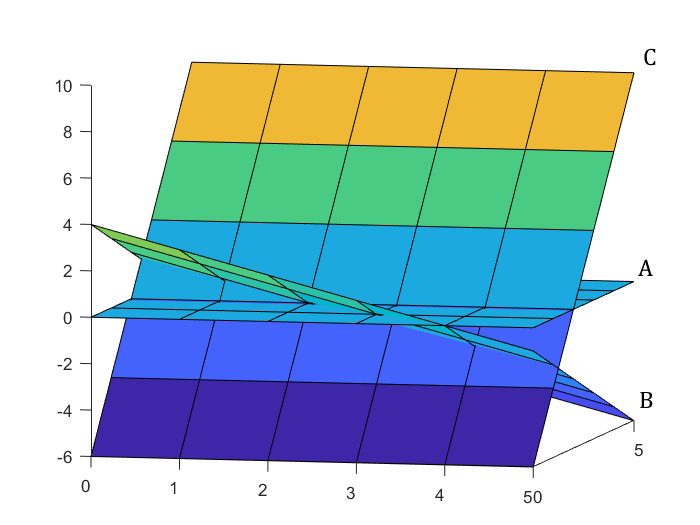
\includegraphics[width=0.6\textwidth]{bounds}
  \caption{Графік функцій обмежень}
  \label{fig:bounds}
\end{figure}

Як видно на графіку, рішення задач $f_1(\vec{x}) \to \max$, $f_2(\vec{x}) \to \max$, $f_3(\vec{x}) \to \max$ є суперечливими та фігура області допустимих значень є замкненою та опуклою.

\subsection{Математична постановка задачі багатокритеріальної оптимізації в загальному вигляді}

У загальному випадку формально задача багатокритеріальної оптимізації, ключовою особливістю якої є суперечливість множини функцій мети (критеріїв), може бути подана в наступному вигляді:
\begin{gather*} 
    f_i(\vec{x}) \to \max, i \in I_1, \\
    f_i(\vec{x}) \to \min, i \in I_2, \\
    \varphi_j(\vec{x}) \leq 0, j \in J.
\end{gather*}
\begin{description}
    \item[де] $I_1$ та $I_2$ --- множини індексів функцій мети $f_i(\vec{x})$, які відповідно максимізуються та мінімізуються, причому $I=I_1 \cup I_2$;
    \item $J$ --- множина індексів функцій $\varphi_j(\vec{x})$, що визначають обмеження задачі та формують множину припустимих варіантів альтернатив $A = \{ \varphi_j(\vec{x}) \leq 0, j \in J \}$;
    \item $\vec{x}$ --- вектор змінних задачі багатокритеріальної оптимізації, з яким пов’яжемо поняття альтернативи --- варіанта розв’язку, що задовольняє обмеження задачі і є способом досягнення поставлених цілей.
\end{description}

\subsection{Математична постановка однокритеріального еквіваленту вихідної багатокритеріальної задачі відповідно до теореми Карлина в загальному вигляді}

Основні положення теореми Карліна формулюються не для первісно заданої множини функцій мети $\{f_i(\vec{x}),i \in I\}$, а для множини функцій $\{\omega_i(\vec{x})=\omega_i(f_i(\vec{x})), i \in I\}$, що складається з монотонних перетворень окремих функцій мети $f_i(\vec{x})$, які приводять їх до безрозмірного вигляду.

Коротко зупинимося на зазначених перетворень. За останні можна взяти одну з монотонних функцій такого вигляду:
\begin{equation}\label{omega1}
\omega^1_i(f_i(\vec{x})) = \systeme[][:]{
\cfrac{f_i^0-f_i(\vec{x})}{f_i^0 - f_{i(\min)}},i \in I_1
:
\cfrac{f_i(\vec{x})-f_i^0}{f_{i(\max)} - f_i^0},i \in I_2
}
,
\end{equation}
\begin{equation}\label{omega2}
\omega^2_i(f_i(\vec{x})) = \systeme[][:]{
\cfrac{f_i^0-f_i(\vec{x})}{f_i^0},i \in I_1
:
\cfrac{f_i(\vec{x})-f_i^0}{f_i^0},i \in I_2
}
,
\end{equation}
\begin{equation}\label{omega3}
\omega^3_i(f_i(\vec{x}))=\omega^j_i(f_i(\vec{x}))^\mu, i \in I, j \in \{1,2\}
.
\end{equation}
\begin{description}
    \item[де] $f_{i(\min)}$, $f_{i(\max)}$ --- найменші і найбільші значення функцій мети, які відповідно максимізуються і мінімізуються на множині припустимих варіантів альтернатив;
    \item $f_i^0$ --- оптимальне значення $i$-ї функції мети на множині припустимих варіантів альтернатив;
    \item $\mu$ --- число, що визначає степінь, на яку підноситься перетворення~\eqref{omega1}~або~\eqref{omega2}.
\end{description}

Згідно теореми Карліна, множина ефективних альтернатив для множини функцій мети $\{f_i(\vec{x}), i \in I\}$ може бути знайдена шляхом розв’язання наступної задачі при використанні відповідних перетворень~\eqref{omega1},~\eqref{omega2}~або~\eqref{omega3}:
\begin{gather*} 
    F(\vec{x}) = \sum_{i \in I}\rho_i\omega^j_i(f_i(\vec{x})) \to \min, \vec{x} \in A, \\
    \sum \rho_i=1, \rho_i > 0, \\ 
    i \in I, j \in \{1,2,3\}.
\end{gather*}
\begin{description}
    \item[де] $\rho_i$ визначає важливість функції мети $f_i(\vec{x})$, і чим більшого значення набуває $\rho_i$, тим кращого значення повинна мати відповідна функція мети.
\end{description}

\subsection{Математична постановка задачі багатокритеріальної оптимізації згідно з виданим завданням}

Згідно виданого завдання задача багатокритеріальної оптимізації прийме наступний вигляд:
Вариант №1

\begin{align*}
k_{u_1}=0.68, k_{u_2}=0.83.
\end{align*}

{
	\small
	\tabulinesep=1.2mm
	\begin{longtabu} to \textwidth {|X[12,l]|X[1,c]X[1,c]X[1,c]|X[1,c]X[1,c]X[1,c]|X[1,c]X[1,c]X[1,c]|X[1,c]X[1,c]X[1,c]|X[1,c]X[1,c]X[1,c]|}  
		\caption{Самооценка экспертов}
		\label{tab:selfscore} \\
		\hline
		\multirow{3}{*}{Источник аргументации} & \multicolumn{15}{c|}{Уровень влияния источника на мнение эксперта} \\ \cline{2-16}
		& \multicolumn{3}{c|}{Эксперт 1} & \multicolumn{3}{c|}{Эксперт 2} & \multicolumn{3}{c|}{Эксперт 3} & \multicolumn{3}{c|}{Эксперт 4} & \multicolumn{3}{c|}{Эксперт 5} \\ \cline{2-16}
		& A & B & C & A & B & C & A & B & C & A & B & C & A & B & C \\ \hline
		\endfirsthead

		\caption*{Окончание таблицы \thetable{}}\\
	    \hline
		\multirow{3}{*}{Источник аргументации} & \multicolumn{15}{c|}{Уровень влияния источника на мнение эксперта} \\ \cline{2-16}
		& \multicolumn{3}{c|}{Эксперт 1} & \multicolumn{3}{c|}{Эксперт 2} & \multicolumn{3}{c|}{Эксперт 3} & \multicolumn{3}{c|}{Эксперт 4} & \multicolumn{3}{c|}{Эксперт 5} \\ \cline{2-16}
		& A & B & C & A & B & C & A & B & C & A & B & C & A & B & C \\ \hline
		\endhead

	 	Проведенный экспертом теоретический анализ данной проблемы 
		& & \checkmark & & & \checkmark & & & \checkmark & & \checkmark & & & & & \checkmark \\ \hline
		Производственный опыт эксперта, связанный с решаемой проблемой & \checkmark & & & & \checkmark & & & \checkmark & & & \checkmark & & & & \checkmark \\ \hline
		Участие в семинарах, совещаниях в своей стране по исследуемой проблеме & & & \checkmark & & & \checkmark & \checkmark & & & & \checkmark & & & \checkmark & \\ \hline
		Знакомство с работами зарубежных авторов по рассматриваемой проблеме & & & \checkmark & & & \checkmark & \checkmark & & & & & \checkmark & & \checkmark & \\ \hline
		Количество проектов, в подготовке, реализации и экспертизе которых эксперт принимал участие & & \checkmark & & & \checkmark & & & \checkmark & & \checkmark & & & & & \checkmark \\ \hline
		Влияние интуиции эксперта на принимаемые решения & & \checkmark & & \checkmark & & & & \checkmark & & & \checkmark & & \checkmark & & \\ \hline
	\end{longtabu}
}

{
	\small
	\tabulinesep=1.2mm
	\begin{longtabu} to \textwidth {|X[1,c]|X[1,c]|X[1,c]|X[1,c]|X[1,c]|X[1,c]|X[1,c]|}  
		\caption{Параметры экспертов}
		\label{tab:score} \\
		\hline
		$k_i$  & $u$ & Эксперт 1 & Эксперт 2 & Эксперт 3 & Эксперт 4 & Эксперт 5 \\ \hline
		\endfirsthead

		\caption*{Окончание таблицы \thetable{}}\\
	    \hline
		$k_i$  & $u$ & Эксперт 1 & Эксперт 2 & Эксперт 3 & Эксперт 4 & Эксперт 5 \\ \hline
		\endhead

	 	$0.0003$ & $u_{lt} $ & $34$ & $26$ & $52$ & $41$ & $60$ \\ \hline
	 	$0.0008$ & $u_{sm} $ & $2$ & $14$ & $15$ & $3$ & $16$ \\ \hline
	 	$0.0015$ & $u_{sd} $ & $16$ & $3$ & $20$ & $21$ & $12$ \\ \hline
	 	$0.0020$ & $u_{z3} $ & $12$ & $14$ & $2$ & $2$ & $32$ \\ \hline
	 	$0.0010$ & $u_{z5} $ & $16$ & $23$ & $24$ & $10$ & $39$ \\ \hline
	 	$0.0009$ & $u_{zsp} $ & $5$ & $2$ & $14$ & $8$ & $9$ \\ \hline
	 	$0.0010$ & $u_{zv} $ & $26$ & $7$ & $2$ & $20$ & $32$ \\ \hline
	 	$0.0015$ & $u_{vs} $ & $5$ & $12$ & $5$ & $2$ & $3$ \\ \hline
	 	$0.0020$ & $u_{vz} $ & $1$ & $2$ & $4$ & $7$ & $0$ \\ \hline
	 	$0.0033$ & $u_{vsp} $ & $18$ & $23$ & $7$ & $21$ & $5$ \\ \hline
	 	$0.0080$ & $u_{zdl} $ & $4$ & $3$ & $5$ & $5$ & $4$ \\ \hline
	 	$0.0070$ & $u_{dlz} $ & $4$ & $3$ & $4$ & $4$ & $4$ \\ \hline
	 	$0.0015$ & $u_{kn} $ & $1$ & $1$ & $1$ & $1$ & $1$ \\ \hline
	 	$0.0200$ & $u_{dn} $ & $0$ & $0$ & $1$ & $1$ & $1$ \\ \hline
	 	$0.0250$ & $u_{zd} $ & $1$ & $0$ & $1$ & $1$ & $1$ \\ \hline
	 	$0.0300$ & $u_{zn} $ & $1$ & $1$ & $1$ & $1$ & $1$ \\ \hline
	 	$0.0350$ & $u_{zpf} $ & $0$ & $0$ & $1$ & $0$ & $1$ \\ \hline
	 	$0.0015$ & $u_{pv} $ & $6$ & $4$ & $15$ & $3$ & $13$ \\ \hline
	 	$0.0018$ & $u_{pn} $ & $2$ & $4$ & $0$ & $6$ & $2$ \\ \hline
	 	$0.0020$ & $u_{ps} $ & $1$ & $0$ & $3$ & $2$ & $8$ \\ \hline
		$0.0250$ & $u_{sk} $ & $0.7$ & $0.65$ & $0.87$ & $0.93$ & $0.84$ \\ \hline
	 	$0.0015$ & $u_{skp} $ & $0.83$ & $0.84$ & $0.79$ & $0.85$ & $0.91$ \\ \hline
	 	$-0.0005$ & $u_{usn} $ & $0$ & $0$ & $0$ & $0$ & $0$ \\ \hline
	 	$0.0003$ & $u_{usi} $ & $0$ & $0$ & $0$ & $0$ & $0$ \\ \hline
	 	$0.0010$ & $u_{usj} $ & $0$ & $0$ & $0$ & $1$ & $0$ \\ \hline
	 	$0.0380$ & $u_{usv} $ & $1$ & $1$ & $1$ & $0$ & $1$ \\ \hline
	 	$0.0100$ & $u_{izp} $ & $5$ & $4$ & $5$ & $5$ & $4$ \\ \hline
	 	$0.0086$ & $u_{ikr} $ & $4$ & $5$ & $5$ & $5$ & $4$ \\ \hline
	 	$-0.0015$ & $u_{iuk} $ & $1$ & $1$ & $2$ & $1$ & $1$ \\ \hline
	 	$0.0100$ & $u_{ilz} $ & $1$ & $0$ & $0$ & $1$ & $1$ \\ \hline
	 	$0.0080$ & $u_{iak} $ & $5$ & $4$ & $3$ & $5$ & $5$ \\ \hline
	\end{longtabu}
}


\subsection{Математична постановка однокритеріального еквіваленту вихідної багатокритеріальної задачі відповідно до теореми Карлина згідно до виданого завдання}

Згідно теореми Карліна для виконання перетворень~\eqref{omega1},~\eqref{omega2},~\eqref{omega3} необхідно знайти мінімальне та максимальне значення окремо для кожної функції мети на допустимій множині альтернатив:
\begin{align*}
    f_{1(\min)}&=0, &   f_{2(\min)}&=0, &   f_{3(\min)}&=0, \\
    f_{1(\max)}&=f_1^0=4,   &   f_{2(\max)}&=f_2^0=2.5, &   f_{3(\max)}&=f_3^0=4.
\end{align*}

Так як мінімальне значення для всіх $f_i$ дорівнюють $0$, то перетворення~\eqref{omega2} буде аналогічне~\eqref{omega1}. Як наслідок, задачі багатокритеріальної оптимізації будуть однакові.

Перетворення~\eqref{omega1},~\eqref{omega2} приймуть наступний вигляд:
\begin{align*}
\omega^{(1,2)}_1(f_1(\vec{x})) &= 
\cfrac{f_1^0-f_1(\vec{x})}{f_1^0 - f_{1(\min)}} =
\cfrac{4 - x_1}{4}, \\
\omega^{(1,2)}_2(f_2(\vec{x})) &= 
\cfrac{f_2^0-f_2(\vec{x})}{f_2^0 - f_{2(\min)}} =
\cfrac{2.5 - x_2}{2.5}, \\
\omega^{(1,2)}_3(f_3(\vec{x})) &= 
\cfrac{f_3^0-f_3(\vec{x})}{f_3^0 - f_{3(\min)}} =
\cfrac{4 - x_3}{4}.
\end{align*}

При використанні перетворень~\eqref{omega1} та~\eqref{omega2} задача матиме вигляд:
\[
F(\vec{x})=\rho_1\cfrac{4 - x_1}{4}+\rho_2\cfrac{2.5 - x_2}{2.5}+\rho_3\cfrac{4 - x_3}{4} \to \min.
\]

При використанні перетвореня~\eqref{omega3}~($\mu = 2$) задача матиме вигляд:
\[
F(\vec{x})=\rho_1\left(\frac{4 - x_1}{4}\right)^2+\rho_2\left(\frac{2.5 - x_2}{2.5}\right)^2+\rho_3\left(\frac{4 - x_3}{4}\right)^2 \to \min.
\]

Результати розрахунків для 3 різних наборів значень вагових коефіцієнтів $\vec{\rho} = (0.7, 0.1, 0.2)$, $\vec{\rho} = (0.3, 0.6, 0.1)$ та $\vec{\rho} = (0.3, 0.3, 0.4)$ були занесені до таблиці~\ref{tab:result}.

    \begin{landscape}% Landscape page
        \begin{table}[H]        
            \caption{Результати розрахунків}
            \label{tab:result}
            \small
        \begin{tabular}{c|c c c|c c c|c c c|c c c|c c c|c}
            % head
            % p
            $j$
            & $\rho_1$   & $\rho_2$   & $\rho_3$ 
            % x
            & $x_1^*$ & $x_2^*$ & $x_3^*$
            % fx
            & $f_1(\vec{x^*})$ & $f_2(\vec{x^*})$ & $f_3(\vec{x^*})$
            % wx
            & $\omega^j_1(\vec{x^*})$ & $\omega^j_2(\vec{x^*})$ & $\omega^j_3(\vec{x^*})$
            % pwx
            & $\rho_1\omega^j_1(\vec{x^*})$ & $\rho_2\omega^j_2(\vec{x^*})$ & $\rho_3\omega^j_3(\vec{x^*})$
            % fx
            & $F(\vec{x^*})$ \\
            \hline

            % 1 first
            \multirow{3}{*}{1}
            % p
            & $0.7$ & $0.1$ & $0.2$ 
            % x
            & $4.0$ & $0.0$ & $0.0$
            % fx
            & $4.0$ & $0.0$ & $0.0$
            % wx
            & $0.0$ & $1.0$ & $1.0$
            % pwx
            & $0.0$ & $0.1$ & $0.2$
            % fx
            & $0.3$ \\

            % 1 two
            % p
            & $0.3$ & $0.6$ & $0.1$ 
            % x
            & $0.0$ & $2.5$ & $1.5$
            % fx
            & $0.0$ & $2.5$ & $1.5$
            % wx
            & $1.0$ & $0.0$ & $0.625$
            % pwx
            & $0.3$ & $0.0$ & $0.0625$
            % fx
            & $0.3625$ \\

            % 1 three
            % p
            & $0.3$ & $0.3$ & $0.4$ 
            % x
            & $0.0$ & $2.5$ & $1.5$
            % fx
            & $0.0$ & $2.5$ & $1.5$
            % wx
            & $1.0$ & $0.0$ & $0.625$
            % pwx
            & $0.3$ & $0.0$ & $0.25$
            % fx
            & $0.55$ \\
            \hline

            % 2 first
            \multirow{3}{*}{2}
            % p
            & $0.7$ & $0.1$ & $0.2$ 
            % x
            & $4.0$ & $0.0$ & $0.0$
            % fx
            & $4.0$ & $0.0$ & $0.0$
            % wx
            & $0.0$ & $1.0$ & $1.0$
            % pwx
            & $0.0$ & $0.1$ & $0.2$
            % fx
            & $0.3$ \\

            % 2 two
            % p
            & $0.3$ & $0.6$ & $0.1$ 
            % x
            & $0.0$ & $2.5$ & $1.5$
            % fx
            & $0.0$ & $2.5$ & $1.5$
            % wx
            & $1.0$ & $0.0$ & $0.625$
            % pwx
            & $0.3$ & $0.0$ & $0.0625$
            % fx
            & $0.3625$ \\

            % 2 three
            % p
            & $0.3$ & $0.3$ & $0.4$ 
            % x
            & $0.0$ & $2.5$ & $1.5$
            % fx
            & $0.0$ & $2.5$ & $1.5$
            % wx
            & $1.0$ & $0.0$ & $0.625$
            % pwx
            & $0.3$ & $0.0$ & $0.25$
            % fx
            & $0.55$ \\
            \hline

            % 3 one
            \multirow{3}{*}{3}
            % p
            & $0.7$ & $0.1$ & $0.2$ 
            % x
            & $3.1015$ & $0.0432$ & $0.8553$
            % fx
            & $3.1015$ & $0.0432$ & $0.8553$
            % wx
            & $0.0505$ & $0.9657$ & $0.618$
            % pwx
            & $0.0353$ & $0.0966$ & $0.1236$
            % fx
            & $0.2555$ \\

            % 3 two
            % p
            & $0.3$ & $0.6$ & $0.1$ 
            % x
            & $2.0$ & $2.0$ & $0.0$
            % fx
            & $2.0$ & $2.0$ & $0.0$
            % wx
            & $0.25$ & $0.04$ & $1.0$
            % pwx
            & $0.075$ & $0.024$ & $0.1$
            % fx
            & $0.199$ \\

            % 3 three
            % p
            & $0.3$ & $0.3$ & $0.4$ 
            % x
            & $0.9635$ & $1.3139$ & $1.7226$
            % fx
            & $0.9635$ & $1.3139$ & $1.7226$
            % wx
            & $0.5763$ & $0.2251$ & $0.3242$
            % pwx
            & $0.1729$ & $0.0675$ & $0.1297$
            % fx
            & $0.3701$ \\
        \end{tabular}
        \end{table}
        \begin{description}
            \item[де] $\vec{x^*}$ --- ефективна альтернатива.
        \end{description}
    \end{landscape}

\subsection{Висновки}

На даній лабораторній роботі було вивчено загальні положення задач багатокритеріальної оптимізації та теорему Карліна про знаходження ефективних альтернатив для багатокритеріальних задач лінійного (нелінійного) програмування. 
Було вирішено задачу багатокритеріальної оптимізації на основі виданого завдання за допомогою  теореми Карліна.

Проаналізуємо отримане рішення задачі однокритеріальної оптимізації при використанні перетворення~\eqref{omega1} та вагових коефіцієнтів $\vec{\rho_1} = (0.7, 0.1, 0.2)$:
була отримана ефективна альтернатива $\vec{x^*} = (4,0,0)$, яка забезпечує досягнення оптимального значення для  функції $f_1(\vec{x^*})$, так як відповідне перетворення дорівнює $0.0$, що свідчить про близькість до оптимуму $f_1(\vec{x^*})$. Отримане рішення відображає наступну закономірність:
\[
\rho_1 \geq \rho_3 \geq \rho_2 \Longrightarrow \omega_1(x^*) \leq \omega_3(x^*) \leq \omega_2(x^*) 
\]

\end{document}

